\poczatekwykladu{11}

\section{Całka po zbiorze miary zero}
\label{sec:calka-po-zbiorze-miary-zero}

Konstrukcja całki przebiegała w trzech etapach. Dla prostej funkcji
nieujemnej całka jest sumą wartości pomnożonych przez miary odpowiednich
zbiorów. Dla funkcji z~$\mathrm{MN}$ bierzemy supremum całek funkcji
prostych leżących pod nią, równoważnie granicę całek niemalejącego
przybliżenia. Dla funkcji dowolnego znaku korzystamy z rozkładu
$f=f^+-f^-$ i definicji~\ref{def:calka-funkcji-mierzalnej}.
Teraz rozważymy własności i przykłady tak otrzymanej całki.

\begin{twierdzenie}
\label{tw:calka-po-zbiorze-miary-zero}
Jeżeli $E\in\mathcal F$, $\mu(E)=0$ i $f\colon X\to\Rbar$ jest
mierzalna, to całka po $E$ istnieje oraz
\[
  \int_E f\,d\mu=0.
\]
\end{twierdzenie}

\begin{proof}
Najpierw niech $f\in\mathrm{PMN}$ oraz
$f=\sum_{i=1}^{m}a_i\mathbf{1}_{A_i}$. Wówczas
\[
  \int_E f\,d\mu
  =\int_X\sum_{i=1}^{m}a_i\mathbf{1}_{A_i\cap E}\,d\mu
  =\sum_{i=1}^{m}a_i\mu(A_i\cap E)=0,
\]
ponieważ $\mu(A_i\cap E)\leq\mu(E)=0$.

Jeżeli $f\in\mathrm{MN}$, to
\[
  \int_E f\,d\mu
  =\sup\left\{\int_X s\,d\mu:
         s\in\mathrm{PMN},\ s\leq f\mathbf{1}_E\right\}.
\]
Każda funkcja $s$ występująca w tym supremum jest zerowa poza $E$.
Ma więc postać $s=s\mathbf{1}_E$ i z pierwszej części dowodu jej
całka jest zerowa. Supremum wynosi zero.

Dla funkcji dowolnego znaku wykorzystujemy tożsamości
\[
  (f\mathbf{1}_E)^+=f^+\mathbf{1}_E,\qquad
  (f\mathbf{1}_E)^-=f^-\mathbf{1}_E.
\]
Obie całki części są zerowe,
zatem $\int_E f\,d\mu=0-0=0$.
\end{proof}

\section{Równość prawie wszędzie a całka}
\label{sec:calka-a-rownosc-prawie-wszedzie}

\begin{twierdzenie}
\label{tw:calka-funkcji-rownych-prawie-wszedzie}
Niech $f,g\colon X\to\Rbar$ będą mierzalne, $E\in\mathcal F$
i $f=g$ $\mu$-prawie wszędzie na $E$. Jeżeli całka
$\int_E f\,d\mu$ istnieje, to całka z $g$ po $E$ także istnieje i
\[
  \int_E f\,d\mu=\int_E g\,d\mu.
\]
W szczególności $f$ jest całkowalna na $E$ wtedy i tylko wtedy,
gdy $g$ jest całkowalna na $E$.
\end{twierdzenie}

\begin{proof}
Niech $F=\{x\in E:f(x)=g(x)\}$. Zbiór $F$ jest mierzalny
i $\mu(E\setminus F)=0$. Addytywność całki funkcji nieujemnej
względem zbioru oraz twierdzenie~\ref{tw:calka-po-zbiorze-miary-zero}
dają
\[
  \int_E f^+\,d\mu
  =\int_F f^+\,d\mu+\int_{E\setminus F}f^+\,d\mu
  =\int_F g^+\,d\mu+0
  =\int_E g^+\,d\mu.
\]
Tak samo $\int_E f^-\,d\mu=\int_E g^-\,d\mu$. Skoro co najmniej
jedna z całek części $f$ jest skończona, to taka sama całka części
$g$ też jest skończona. Różnice określające obie całki są więc
poprawnie zdefiniowane i równe. Skończoność obu całek części
przenosi się z jednej funkcji na drugą.
\end{proof}

\section{Przykłady całek i sumy miar}
\label{sec:przyklady-calki-i-sumy-miar}

\begin{przyklad}[Miara Diraca]
\label{prz:calka-wzgledem-diraca}
Niech $x_0\in X$, a $\delta_{x_0}$ będzie miarą skupioną w $x_0$
na przestrzeni mierzalnej $(X,\mathcal F)$. Dla każdej mierzalnej
funkcji $f\colon X\to\R$ mamy
\begin{equation}
  \int_X f\,d\delta_{x_0}=f(x_0).
  \label{eq:calka-wzgledem-diraca}
\end{equation}
Dla funkcji prostej $s=\sum_i a_i\mathbf{1}_{A_i}$ wynika to z równości
\[
  \int_X s\,d\delta_{x_0}
  =\sum_i a_i\delta_{x_0}(A_i)
  =\sum_i a_i\mathbf{1}_{A_i}(x_0)=s(x_0).
\]
Przybliżając funkcję nieujemną od dołu funkcjami prostymi, dostajemy
tę samą równość dla $f\in\mathrm{MN}$. Dla rzeczywistej funkcji
dowolnego znaku całki części są równe $f^+(x_0)$ i $f^-(x_0)$.
Obie są skończone, a ich różnica wynosi $f(x_0)$.

Jeżeli singleton $\{x_0\}$ jest mierzalny, można też rozbić całkę na
całki po $\{x_0\}$ i $X\setminus\{x_0\}$. Druga jest zerowa, zaś
na pierwszym zbiorze $f$ ma stałą wartość $f(x_0)$.
\end{przyklad}

\begin{przyklad}[Dwa punkty o różnych wagach]
\label{prz:calka-miara-dwupunktowa}
Ustalmy różne punkty $x_1,x_2\in X$ i miarę
$\mu=\delta_{x_1}+2\delta_{x_2}$. Dla $A\in\mathcal F$ mamy
\[
  \mu(A)=
  \begin{cases}
    1, & x_1\in A,\ x_2\notin A,\\
    2, & x_1\notin A,\ x_2\in A,\\
    3, & x_1,x_2\in A,\\
    0, & x_1,x_2\notin A.
  \end{cases}
\]
Jest to miara, ponieważ każda z miar Diraca jest przeliczalnie
addytywna, a sumowanie dwóch nieujemnych szeregów można wykonać
składnikami. Dla mierzalnej $f\colon X\to\R$ otrzymujemy
\[
  \int_X f\,d\mu=f(x_1)+2f(x_2).
\]
Dla funkcji prostej wynika to bezpośrednio z sumy definiującej całkę,
dla nieujemnej z przybliżenia funkcjami prostymi, a dla funkcji obu
znaków z rozkładu na części. Schemat dwóch wag przedstawia
rysunek~\ref{fig:miara-atomowa-dwupunktowa}.
\end{przyklad}

\begin{figure}[htbp]
  \centering
  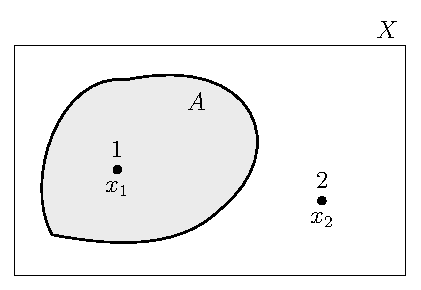
\includegraphics[width=0.48\textwidth]{miara-atomowa-dwupunktowa.pdf}
  \caption{Miara $\delta_{x_1}+2\delta_{x_2}$ przypisuje punktom wagi $1$ i $2$. Dla narysowanego zbioru $A$ mamy $\mu(A)=1$.}
  \label{fig:miara-atomowa-dwupunktowa}
\end{figure}

\begin{fakt}[Całka względem sumy miar]
\label{fakt:calka-wzgledem-sumy-miar}
Jeżeli $\mu_1,\ldots,\mu_r$ są miarami na $(X,\mathcal F)$, to
\[
  \mu(A)=\mu_1(A)+\cdots+\mu_r(A),\qquad A\in\mathcal F,
\]
też jest miarą. Dla $f\in\mathrm{MN}$ zachodzi
\begin{equation}
  \int_X f\,d\mu=\sum_{i=1}^{r}\int_X f\,d\mu_i.
  \label{eq:calka-wzgledem-sumy-miar}
\end{equation}
Dla mierzalnej funkcji dowolnego znaku równość ta zachodzi,
jeżeli całka po lewej stronie istnieje. Wszystkie całki po prawej
stronie są wówczas określone, a ich suma też jest określona.
\end{fakt}

\begin{proof}
Przeliczalna addytywność $\mu$ wynika z zamiany kolejności skończonej
sumy i szeregu o wyrazach nieujemnych. Dla
$s=\sum_{j=1}^{m}a_j\mathbf{1}_{A_j}\in\mathrm{PMN}$ mamy
\[
  \int_X s\,d\mu
  =\sum_{j=1}^{m}a_j\sum_{i=1}^{r}\mu_i(A_j)
  =\sum_{i=1}^{r}\int_X s\,d\mu_i.
\]
Jeśli $s_n\in\mathrm{PMN}$ i $s_n\uparrow f$, twierdzenie
o zbieżności monotonicznej daje
\[
  \int_X f\,d\mu
  =\lim_{n\to\infty}\sum_{i=1}^{r}\int_X s_n\,d\mu_i
  =\sum_{i=1}^{r}\int_X f\,d\mu_i.
\]
Granica skończonej sumy nieujemnych, niemalejących składników jest
sumą ich granic, także przy wartościach nieskończonych.

Dla funkcji obu znaków stosujemy tę równość do $f^+$ i $f^-$.
Co najmniej jedna z sum całek części jest skończona, więc wszystkie
jej składniki są skończone. Możemy zatem odjąć te sumy składnikami,
otrzymując~\eqref{eq:calka-wzgledem-sumy-miar}.
\end{proof}

\begin{przyklad}[Miara licząca i szeregi]
\label{prz:calka-miara-liczaca}
Rozważmy $(\{1,2,\ldots\},\mathcal P(\{1,2,\ldots\}),\eta)$,
gdzie $\eta(A)=|A|$ dla zbiorów skończonych i $\eta(A)=+\infty$
dla zbiorów nieskończonych. Każda funkcja na tej przestrzeni jest
mierzalna. Jeżeli $f\geq0$, kładziemy
\[
  s_n(m)=
  \begin{cases}
    f(m), & m\leq n,\\
    0, & m>n.
  \end{cases}
\]
Dla skończonych wartości $f(m)$ każda $s_n$ jest funkcją prostą,
$s_n\uparrow f$ oraz
\[
  \int s_n\,d\eta=\sum_{m=1}^{n}f(m)\eta(\{m\})
               =\sum_{m=1}^{n}f(m).
\]
Stąd
\begin{equation}
  \int f\,d\eta=\lim_{n\to\infty}\sum_{m=1}^{n}f(m)
              =\sum_{m=1}^{\infty}f(m).
  \label{eq:calka-miara-liczaca}
\end{equation}
Dla $f$ przyjmującej wartość $+\infty$ w którymś punkcie obie strony
są nieskończone, co wynika także z monotoniczności całki.
Przybliżenie $s_n$ ilustruje rysunek~\ref{fig:calka-miara-liczaca}.

Podobnie, dla miary liczącej na $\mathbb Z$,
\[
  \int_{\mathbb Z}f\,d\eta=\sum_{n\in\mathbb Z}a_n,
  \qquad f(n)=a_n\geq0.
\]
Dla wyrazów obu znaków całka istnieje wtedy i tylko wtedy, gdy
co najmniej jeden z szeregów $\sum a_n^+$, $\sum a_n^-$ jest
skończony. Całkowalność jest równoważna $\sum |a_n|<+\infty$.
Tak samo interpretujemy wzór~\eqref{eq:calka-miara-liczaca}
dla funkcji obu znaków.
\end{przyklad}

\begin{figure}[htbp]
  \centering
  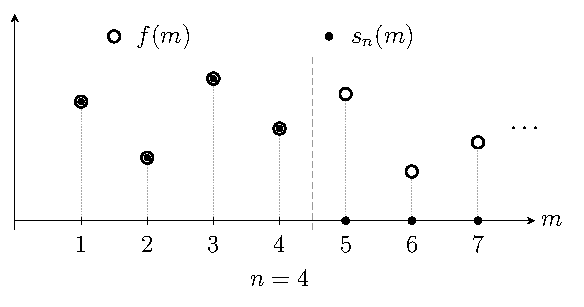
\includegraphics[width=0.76\textwidth]{calka-miara-liczaca.pdf}
  \caption{Przybliżenie $s_n$ zachowuje pierwszych $n$ wartości funkcji $f$ i zeruje pozostałe. Na schemacie $n=4$.}
  \label{fig:calka-miara-liczaca}
\end{figure}

\begin{samepage}
\section{Całka Riemanna a całka Lebesgue'a}
\label{sec:calka-riemanna-a-lebesguea}

\begin{twierdzenie}
\label{tw:riemann-lebesgue}
Jeżeli $a<b$, a $f\colon[a,b]\to\R$ jest ograniczona i całkowalna
w sensie Riemanna, to $f$ jest mierzalna względem sigma-ciała
Lebesgue'a, całkowalna względem miary Lebesgue'a $\lambda$ oraz
\begin{equation}
  \int_a^b f(x)\,dx=\int_{[a,b]}f\,d\lambda.
  \label{eq:riemann-lebesgue}
\end{equation}
Po lewej stronie występuje całka Riemanna.
\end{twierdzenie}
\end{samepage}

\begin{uwaga}[Funkcja Dirichleta]
\label{uw:dirichlet-calka-riemanna}
Funkcja $D=\mathbf{1}_{\mathbb Q}$ jest borelowska i
$\int_{\R}D\,d\lambda=\lambda(\mathbb Q)=0$. Na każdym odcinku
$[a,b]$ z $a<b$ jej dolna suma Darboux wynosi zero, a górna
$b-a$, ponieważ każdy przedział o dodatniej długości zawiera liczby
wymierne i niewymierne. Funkcja $D$ nie jest więc całkowalna
w sensie Riemanna na takim odcinku. Funkcje całkowalne Riemanna
na $[a,b]$ tworzą właściwy podzbiór funkcji całkowalnych Lebesgue'a
na $[a,b]$.
\end{uwaga}

\begin{przyklad}[Całka niewłaściwa a całka Lebesgue'a]
\label{prz:calka-niewlasciwa-nieistnienie-lebesguea}
Niech dla $n=0,1,2,\ldots$
\[
  f(x)=
  \begin{cases}
    \dfrac{1}{n+1}, & x\in[2n,2n+1),\\[4pt]
    -\dfrac{1}{n+1}, & x\in[2n+1,2n+2),\\[4pt]
    0, & x<0.
  \end{cases}
\]
Jest to funkcja borelowska, przedstawiona na
rysunku~\ref{fig:calka-schodkowa-niewlasciwa}.
Na każdym skończonym odcinku $[0,t]$ jest całkowalna Riemanna.
Całka po każdym bloku $[2n,2n+2]$ wynosi zero. Jeżeli
$t\in[2n,2n+2]$, to
\[
  \left|\int_0^t f(x)\,dx\right|\leq\frac{1}{n+1}.
\]
Zatem całka niewłaściwa istnieje i
\[
  \int_0^\infty f(x)\,dx
  :=\lim_{t\to+\infty}\int_0^t f(x)\,dx=0.
\]
Jednocześnie z twierdzenia o zbieżności monotonicznej zastosowanego
do kolejnych sum części nieujemnych wynika
\[
  \int_{[0,+\infty)}f^+\,d\lambda
  =\sum_{n=0}^{\infty}\frac{1}{n+1}=+\infty,\qquad
  \int_{[0,+\infty)}f^-\,d\lambda=+\infty.
\]
Całka Lebesgue'a z $f$ po $[0,+\infty)$ jest więc nieokreślona.
\end{przyklad}

\begin{figure}[htbp]
  \centering
  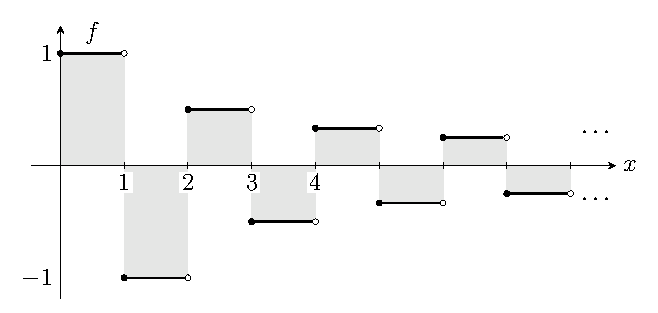
\includegraphics[width=0.85\textwidth]{calka-schodkowa-niewlasciwa.pdf}
  \caption{Dodatnie i ujemne bloki o długości $1$ mają przeciwne całki. Ich wysokości maleją jak $1/(n+1)$.}
  \label{fig:calka-schodkowa-niewlasciwa}
\end{figure}

\begin{proof}[Dowód twierdzenia~\ref{tw:riemann-lebesgue}]
Zacznijmy od $0\leq f\leq M$. Dla podziału
$P=(a=x_0<x_1<\cdots<x_k=b)$ kładziemy
\[
  m_i=\inf_{x\in[x_{i-1},x_i]}f(x),\qquad
  M_i=\sup_{x\in[x_{i-1},x_i]}f(x).
\]
Sumy Darboux mają postać
\[
  L(f,P)=\sum_{i=1}^{k}m_i(x_i-x_{i-1}),\qquad
  U(f,P)=\sum_{i=1}^{k}M_i(x_i-x_{i-1}).
\]
Na rozłącznych przedziałach $I_1=[a,x_1]$ oraz
$I_i=(x_{i-1},x_i]$ dla $i\geq2$ definiujemy funkcje proste
\[
  s_P=\sum_{i=1}^{k}m_i\mathbf{1}_{I_i},\qquad
  t_P=\sum_{i=1}^{k}M_i\mathbf{1}_{I_i}.
\]
Wtedy $s_P\leq f\leq t_P$ punktowo i
\[
  \int_{[a,b]}s_P\,d\lambda=L(f,P),\qquad
  \int_{[a,b]}t_P\,d\lambda=U(f,P).
\]
Przydzielenie końców odcinków do rozłącznych części zachowuje ich
długości. Schemat przedstawia rysunek~\ref{fig:sumy-darboux}.

Uzasadnijmy mierzalność $f$. Całkowalność Riemanna pozwala wybrać
podziały $P_n$ z $U(f,P_n)-L(f,P_n)\to0$. Funkcje
\[
  l=\sup_n s_{P_n},\qquad u=\inf_n t_{P_n}
\]
są mierzalne, ograniczone i spełniają $l\leq f\leq u$. Stąd
\[
  0\leq\int_{[a,b]}(u-l)\,d\lambda
  \leq U(f,P_n)-L(f,P_n)\longrightarrow0.
\]
Dla każdego $j\geq1$ monotoniczność całki daje
$\lambda(\{u-l\geq1/j\})/j\leq\int_{[a,b]}(u-l)\,d\lambda=0$.
Zatem $N=\{u>l\}$ jest mierzalnym zbiorem miary zero. Poza $N$
mamy $f=l$. Zupełność miary Lebesgue'a zapewnia mierzalność $f$,
ponieważ każdy zbiór $\{f>c\}$ różni się od mierzalnego
$\{l>c\}$ jedynie na podzbiorze $N$.

\begin{samepage}
Oznaczmy przez $L_D(f)=\sup_P L(f,P)$ i $U_D(f)=\inf_P U(f,P)$
dolną i górną całkę Darboux, a przez $I$ całkę Lebesgue'a z $f$
po $[a,b]$. Z definicji całki nieujemnej i monotoniczności mamy
\[
  L_D(f)\leq I
  \leq\inf_{\substack{t\in\mathrm{PMN}\\t\geq f}}
                   \int_{[a,b]}t\,d\lambda
  \leq U_D(f).
\]
Funkcje proste w tym wzorze rozważamy na $[a,b]$.
Ponieważ $f$ jest całkowalna w sensie Riemanna,
$L_D(f)=U_D(f)=\int_a^b f(x)\,dx$, co daje równość~\eqref{eq:riemann-lebesgue}.
\end{samepage}

Oszacowanie od góry otrzymujemy także z oszacowania od dołu
dla $g=M-f\geq0$. Wówczas
\[
  L_D(g)=M(b-a)-U_D(f)
  \leq\int_{[a,b]}g\,d\lambda=M(b-a)-I,
\]
a więc $I\leq U_D(f)$.

Dla funkcji obu znaków wybieramy $C\geq0$ takie, że $f+C\geq0$.
Funkcja $f+C$ jest ograniczona i całkowalna w sensie Riemanna,
więc poprzednia część dowodu stosuje się do niej. Odejmując
$C(b-a)$ po obu stronach równości całek, otrzymujemy wynik dla $f$.
Ograniczoność na odcinku o skończonej długości daje całkowalność
w sensie Lebesgue'a.
\end{proof}

\begin{figure}[htbp]
  \centering
  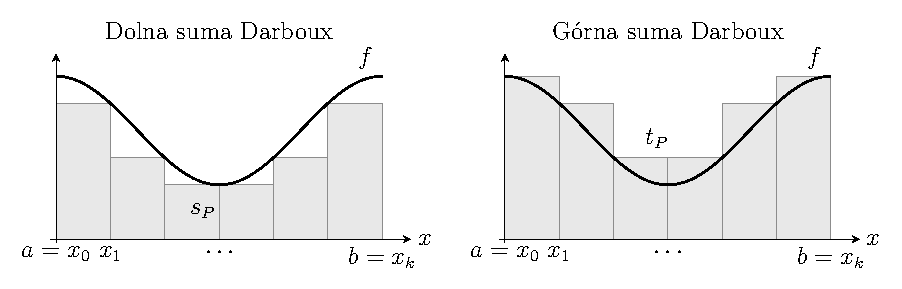
\includegraphics[width=0.98\textwidth]{sumy-darboux.pdf}
  \caption{Dolna i górna suma Darboux jako całki funkcji prostych $s_P\leq f\leq t_P$.}
  \label{fig:sumy-darboux}
\end{figure}
